% !TEX root = RailVehicleIntroduction.tex
\section{Rail vehicle fundamentals}
\subsection{Rail vehicle structure}

\frame{\frametitle{Structural elements}
\begin{center}
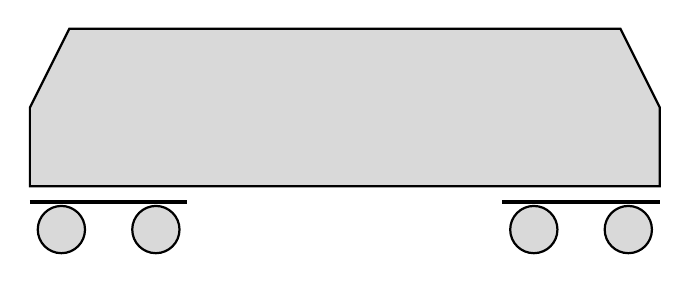
\begin{tikzpicture}
\draw[thick, fill = gray!30] (0,0) -- (0,1) -- (.5,2) -- (7.5,2) -- (8,1) -- (8,0) -- cycle;
\draw[ultra thick] (0, -.2) -- (2, -.2); 
\draw[thick, fill = gray!30] (.4, -.55) circle (.3);
\draw[thick, fill = gray!30] (1.6, -.55) circle (.3);
\begin{scope} [shift = {(6,0)}]
\draw[ultra thick] (0, -.2) -- (2, -.2); 
\draw[thick, fill = gray!30] (.4, -.55) circle (.3);
\draw[thick, fill = gray!30] (1.6, -.55) circle (.3);
\end{scope}
\end{tikzpicture}
\end{center}
}

\subsection{Operating conditions}
\frame{\frametitle{Comparison of road and rail vehicles \footnote{Minde, IVE Hannover, 2007}}
\begin{small}
\begin{tabular}{|p{5cm}|p{5cm}|}
  \hline                       
Friction coefficient rubber-road ($\mu_H \approx 0,9$) & Friction coefficient steel-steel ($\mu_H \approx 0,15$)  \\ \hline
Small axle load ($m_{al} \approx 0,8 t$) & High axle load ($m_{al} \approx 20 t$)  \\ \hline
Short braking distance & Long braking distance  \\ \hline
Two coupled vehicles at maximum & Formation of trains  \\ \hline
Evading possible & Track guidance  \\ \hline
On-sight control & Signalling  \\ \hline
Relative braking distance & Absolute braking distance  \\ \hline
Direct feedback of brake & Delayed brake action  \\
  \hline  
\end{tabular}
\end{small}
}

\frame{\frametitle{Conditions}
\begin{columns}[t] % contents are top vertically aligned
     \begin{column}[T]{6cm} % each column can also be its own environment
     \begin{itemize}
     \item \glqq Good conditions\grqq \ comparable to \glqq extreme conditions\grqq \ on the road
     \end{itemize}
		Try your own calculation using WolframAlpha or online here: http://www.auburn.nsw.gov.au/ Explore/RoadSafety/ RoadSafetyDocuments/ calculator.html
     \end{column}
     \begin{column}[T]{5cm} % alternative top-align that's better for graphics
         \begin{center}
            \includegraphics[width=0.7\textwidth]{Bremsweg2}
        \end{center}
     \end{column}
     \end{columns}
}

\frame{\frametitle{Main features of rail vehicles}
\framesubtitle{}
\vspace{-.5cm}
\begin{center}
\scriptsize
\begin{tabular}{|p{.8cm}|p{1.3cm}|p{1.3cm}|p{1.3cm}|p{1.3cm}|p{1.5cm}|p{1.3cm}|}
\hline
 & Tram & Light rail & Metro & Suburban & Conventional & Highspeed \\ \hline
Track & On Road & Widely separated & Fully separated & Main line & Main line & Main line, partly dedicated \\ \hline
Curve radius & $\geq 15\mathrm{m}$ & $\geq 25\mathrm{m}$ & $\geq 90\mathrm{m}$ & $\geq 180\mathrm{m}$ & $\geq 625\mathrm{m}$ & $\geq 1800\mathrm{m}$ \\ \hline
Train protection & On Sight & Sight/ Signals & Signals & Signals & Signals & Drivers desk signalling \\ \hline
$d_{Stops}$ & $(300 \ldots$ $ 600)\mathrm{m}$ & $(500 \ldots $ $ 800)\mathrm{m}$ & $(500 \ldots $ $ 1000)\mathrm{m}$ & $(750 \ldots $ $ 3000)\mathrm{m}$ & $(3 \ldots $ $20)\mathrm{km}$ & $\gg 20\mathrm{km} $ \\ \hline
Vehicle length  & $(20 \ldots 53)\mathrm{m}$ & $(25 \ldots  40)\mathrm{m}$ & $(25 \ldots  40)\mathrm{m}$ & $(25 \ldots  40)\mathrm{m}$ & $\approx 26 \mathrm{m}$ & $ \approx 26 (28)\mathrm{m} $ \\ \hline
Train length & $\leq 75 \mathrm{m}$ & $ \leq 75\mathrm{m}$ & $\leq 120\mathrm{m}$ & $\leq 300 \mathrm{m}$ & $\leq 400 \mathrm{m}$ & $ \leq 400 \mathrm{m} $ \\ \hline
$v_{max}$  & $70 \mathrm{km/h}$ & $ 100\mathrm{km/h}$ & $100 \mathrm{km/h}$ & $140 \mathrm{km/h}$ & $\leq 189 \mathrm{km/h}$ & $ \geq 190 \mathrm{km/h} $ \\ \hline
$a_{max}$ & $\leq 1.5 \frac{\mathrm{m}}{\mathrm{s}^2}$ & $\leq 1.5 \frac{\mathrm{m}}{\mathrm{s}^2}$ & $\leq 1.3 \frac{\mathrm{m}}{\mathrm{s}^2}$ & $\leq 1.15 \frac{\mathrm{m}}{\mathrm{s}^2}$ & $\leq 1.15 \frac{\mathrm{m}}{\mathrm{s}^2}$ & $\leq 1.15 \frac{\mathrm{m}}{\mathrm{s}^2}$ \\ \hline
$b_{max}$ & $\leq 3 \frac{\mathrm{m}}{\mathrm{s}^2}$ & $\leq 3 \frac{\mathrm{m}}{\mathrm{s}^2}$ & $\leq 1.3 \frac{\mathrm{m}}{\mathrm{s}^2}$ & $\leq 1.0 \frac{\mathrm{m}}{\mathrm{s}^2}$ & $\leq 1.5 \frac{\mathrm{m}}{\mathrm{s}^2}$ & $\leq 1.5 \frac{\mathrm{m}}{\mathrm{s}^2}$ \\ \hline
$F_{L, test}$ & $\leq 300 \mathrm{kN}$ & $\leq 600 \mathrm{kN}$ & $\leq 800 \mathrm{kN}$ & $\leq 1500 \mathrm{kN}$ & $\leq 1500 \mathrm{kN}$ & $\leq 1500 \mathrm{kN}$ \\ \hline
\end{tabular}
\end{center}
}




